\documentclass[12pt,]{article}
\usepackage{lmodern}
\usepackage{amssymb,amsmath}
\usepackage{ifxetex,ifluatex}
\usepackage{fixltx2e} % provides \textsubscript
\ifnum 0\ifxetex 1\fi\ifluatex 1\fi=0 % if pdftex
  \usepackage[T1]{fontenc}
  \usepackage[utf8]{inputenc}
\else % if luatex or xelatex
  \ifxetex
    \usepackage{mathspec}
  \else
    \usepackage{fontspec}
  \fi
  \defaultfontfeatures{Ligatures=TeX,Scale=MatchLowercase}
\fi
% use upquote if available, for straight quotes in verbatim environments
\IfFileExists{upquote.sty}{\usepackage{upquote}}{}
% use microtype if available
\IfFileExists{microtype.sty}{%
\usepackage{microtype}
\UseMicrotypeSet[protrusion]{basicmath} % disable protrusion for tt fonts
}{}
\usepackage[margin=1in]{geometry}
\usepackage{hyperref}
\hypersetup{unicode=true,
            pdfborder={0 0 0},
            breaklinks=true}
\urlstyle{same}  % don't use monospace font for urls
\usepackage{graphicx,grffile}
\makeatletter
\def\maxwidth{\ifdim\Gin@nat@width>\linewidth\linewidth\else\Gin@nat@width\fi}
\def\maxheight{\ifdim\Gin@nat@height>\textheight\textheight\else\Gin@nat@height\fi}
\makeatother
% Scale images if necessary, so that they will not overflow the page
% margins by default, and it is still possible to overwrite the defaults
% using explicit options in \includegraphics[width, height, ...]{}
\setkeys{Gin}{width=\maxwidth,height=\maxheight,keepaspectratio}
\IfFileExists{parskip.sty}{%
\usepackage{parskip}
}{% else
\setlength{\parindent}{0pt}
\setlength{\parskip}{6pt plus 2pt minus 1pt}
}
\setlength{\emergencystretch}{3em}  % prevent overfull lines
\providecommand{\tightlist}{%
  \setlength{\itemsep}{0pt}\setlength{\parskip}{0pt}}
\setcounter{secnumdepth}{0}
% Redefines (sub)paragraphs to behave more like sections
\ifx\paragraph\undefined\else
\let\oldparagraph\paragraph
\renewcommand{\paragraph}[1]{\oldparagraph{#1}\mbox{}}
\fi
\ifx\subparagraph\undefined\else
\let\oldsubparagraph\subparagraph
\renewcommand{\subparagraph}[1]{\oldsubparagraph{#1}\mbox{}}
\fi

%%% Use protect on footnotes to avoid problems with footnotes in titles
\let\rmarkdownfootnote\footnote%
\def\footnote{\protect\rmarkdownfootnote}

%%% Change title format to be more compact
\usepackage{titling}

% Create subtitle command for use in maketitle
\newcommand{\subtitle}[1]{
  \posttitle{
    \begin{center}\large#1\end{center}
    }
}

\setlength{\droptitle}{-2em}
  \title{\Large{"Revisiting the Biological Value Index (Sanders, 1960), Contribution to its calculation and visualization"}}
  \pretitle{\vspace{\droptitle}\centering\huge}
  \posttitle{\par}
  \author{}
  \preauthor{}\postauthor{}
  \date{}
  \predate{}\postdate{}

\usepackage{booktabs}
\usepackage{longtable}
\usepackage{array}
\usepackage{multirow}
\usepackage[table]{xcolor}
\usepackage{wrapfig}
\usepackage{setspace}
\doublespacing
\usepackage{lineno}
\linenumbers

\begin{document}
\maketitle

Juan Carlos Villaseñor-Derbez\textsuperscript{1}, Arturo
Ramírez-Valdez\textsuperscript{2}

\textsuperscript{1}Bren School of Environmental Science \& Management
University of California at Santa Barbara, Santa Barbara, California,
USA

\textsuperscript{2}SCRIPPS Institution of Oceanography, University of
California at San Diego, San Diego, California, USA

Corresponding author: Juan Carlos Villaseñor-Derbez\textsuperscript{1}

Email address:\\
\href{mailto:jvillasenor@bren.ucsb.edu}{\nolinkurl{jvillasenor@bren.ucsb.edu}}

\clearpage

Abstract: No more than approx. 500 words (or 3,000 characters).

\section{Introduction}\label{introduction}

\begin{itemize}
\item
  Indices in ecology
\item
  History of the index

  \begin{itemize}
  \tightlist
  \item
    When it was proposed
  \item
    How it worked
  \item
    Modifications by Loya Salinas
  \item
    How it works now
  \end{itemize}
\item
  Usage of the index

  \begin{itemize}
  \tightlist
  \item
    Works that have used it
  \end{itemize}
\item
  Stating the problem

  \begin{itemize}
  \tightlist
  \item
    Lack of comparison
  \item
    computability
  \end{itemize}
\end{itemize}

\section{Materials and Methods}\label{materials-and-methods}

\begin{itemize}
\item
  How the index works, step by step (possibly citing Loya-Salinas)
\item
  Flow diagram depfun(ivb)
\item
  Adding the \%BVI
\end{itemize}

\begin{equation}\%BVI_i = \frac{(100\times BVI_i)}{\sum_{i = 1}^nBVI_i}\end{equation}

\begin{itemize}
\item
  Compare N and Ni vs rBVI to test its usefulness
\item
  Propose ways to visualize rBVI
\item
  Recreating Loya-Salinas
\end{itemize}

\begin{tabular}{>{\em}lrrrrrr}
\toprule
Spp & S1 & S2 & S3 & S4 & S5 & S6\\
\midrule
Synchelidium spp. & 2398 & 1626 & 811 & 1275 & 1343 & 7079\\
Tridentella spp. & 2048 & 1125 & 528 & 1990 & 1098 & 1274\\
Nerine cirratulus & 37 & 165 & 1141 & 1540 & 118 & 53\\
Nephtys californiensis & 544 & 875 & 404 & 170 & 58 & 90\\
Glycera tenuis & 265 & 566 & 106 & 646 & 133 & 118\\
\addlinespace
Donax gouldii & 914 & 75 & 42 & 5 & 5 & 15\\
Orchestoidea benedicti & 11 & 251 & 133 & 79 & 162 & 245\\
Archaeomysis spp. & 958 & 90 & 160 & 37 & 522 & 111\\
Armadillium spp. & 59 & 155 & 91 & 16 & 208 & 283\\
Megalopus spp. & 149 & 266 & 48 & 30 & 0 & 0\\
\addlinespace
Emerita analoga & 101 & 16 & 96 & 27 & 0 & 10\\
Pontharpinia spp. & 69 & 96 & 11 & 16 & 0 & 0\\
Euzonus mucronata & 0 & 0 & 37 & 341 & 0 & 0\\
Lepidopa californica & 5 & 69 & 16 & 0 & 16 & 0\\
Magelona californica & 0 & 5 & 5 & 0 & 42 & 10\\
\addlinespace
Hanstorina spp. & 0 & 16 & 5 & 0 & 0 & 0\\
Glycera dibranchiata & 0 & 0 & 0 & 0 & 5 & 0\\
Archaeomysis maculata & 0 & 0 & 0 & 5 & 0 & 0\\
\bottomrule
\end{tabular}

\begin{itemize}
\tightlist
\item
  Mention using SIMPER as a comparative
\item
  Propose a graph to visualize data
\end{itemize}

\section{Results}\label{results}

\begin{itemize}
\tightlist
\item
  Results from Loya-Salinas
\item
  Graph
\item
  Comparing \%BVI with SIMPER
\item
  Table with abundances, BVI, \%BVI and SIMPER
\end{itemize}

\begin{tabular}{>{\em}llllllllr}
\toprule
Species & S1 & S2 & S3 & S4 & S5 & S6 & BVI & \%BVI\\
\midrule
Synchelidium spp. & 10 & 10 & 9 & 8 & 10 & 10 & 57 & 17.22\\
Tridentella spp. & 9 & 9 & 8 & 10 & 9 & 9 & 54 & 16.31\\
Glycera tenuis & 5 & 7 & 4 & 7 & 5 & 6 & 34 & 10.27\\
Nephtys californiensis & 6 & 8 & 7 & 5 & 3 & 4 & 33 & 9.97\\
Archaeomysis spp. & 8 & 1 & 6 & 3 & 8 & 5 & 31 & 9.37\\
\addlinespace
Nerine cirratulus & 0 & 4 & 10 & 9 & 4 & 3 & 30 & 9.06\\
Orchestoidea benedicti & 0 & 5 & 5 & 4 & 6 & 7 & 27 & 8.16\\
Armadillium spp. & 1 & 3 & 2 & 0 & 7 & 8 & 21 & 6.34\\
Megalopus spp. & 4 & 6 & 1 & 2 & 0 & 0 & 13 & 3.93\\
Donax gouldii & 7 & 0 & 0 & 0 & 0 & 2 & 9 & 2.72\\
\addlinespace
Others & 5 & 2 & 3 & 7 & 3 & 2 & 22 & 0.07\\
Total &  &  &  &  &  &  &  & 100.00\\
\bottomrule
\end{tabular}

\begin{table}[!htbp] \centering 
  \caption{} 
  \label{} 
\begin{tabular}{@{\extracolsep{5pt}}lcc} 
\\[-1.8ex]\hline 
\hline \\[-1.8ex] 
 & \multicolumn{2}{c}{\textit{Dependent variable:}} \\ 
\cline{2-3} 
\\[-1.8ex] & Abundance & RelAbundance \\ 
\\[-1.8ex] & (1) & (2)\\ 
\hline \\[-1.8ex] 
 rBVI & 0.118$^{***}$ (0.010) & 0.016$^{***}$ (0.002) \\ 
  Constant & 1.189$^{***}$ (0.090) & $-$0.040$^{**}$ (0.016) \\ 
 \hline \\[-1.8ex] 
Observations & 81 & 81 \\ 
R$^{2}$ & 0.636 & 0.489 \\ 
Adjusted R$^{2}$ & 0.632 & 0.482 \\ 
Residual Std. Error (df = 79) & 0.482 & 0.088 \\ 
F Statistic (df = 1; 79) & 138.264$^{***}$ & 75.486$^{***}$ \\ 
\hline 
\hline \\[-1.8ex] 
\textit{Note:}  & \multicolumn{2}{r}{$^{*}$p$<$0.1; $^{**}$p$<$0.05; $^{***}$p$<$0.01} \\ 
\end{tabular} 
\end{table}

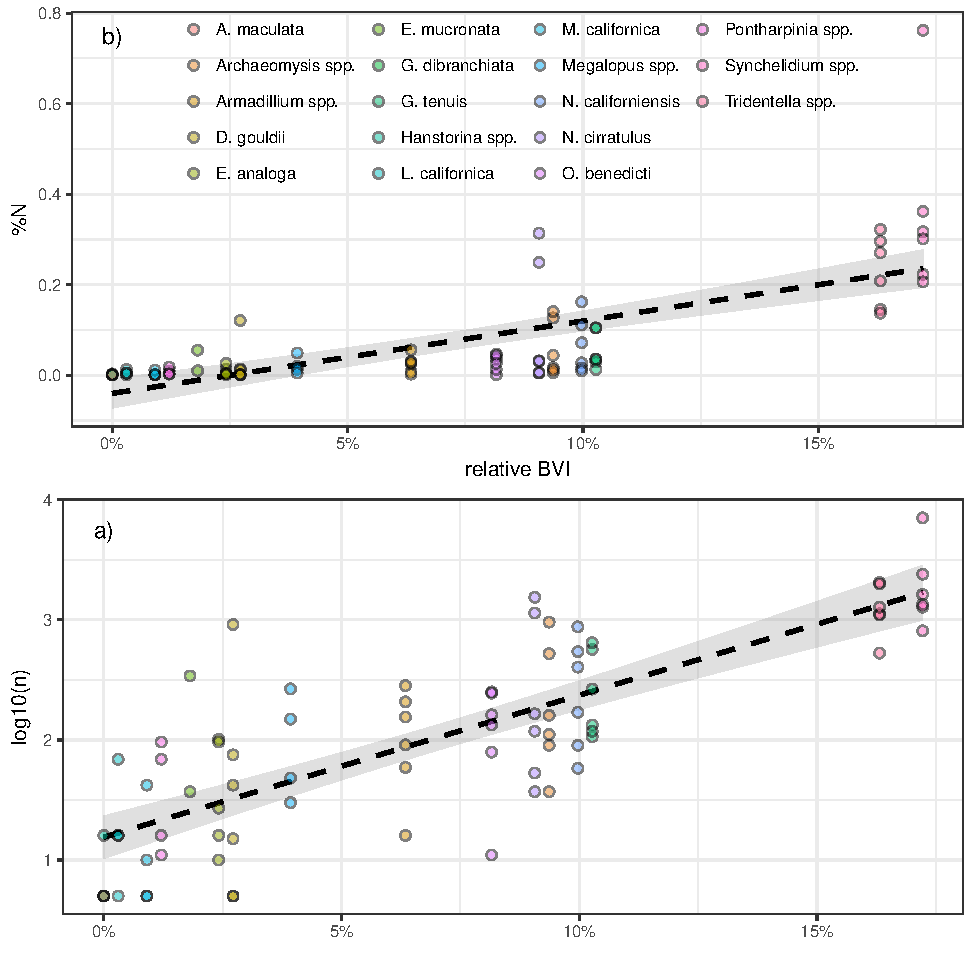
\includegraphics{BVI_Manuscript_files/figure-latex/unnamed-chunk-7-1.pdf}

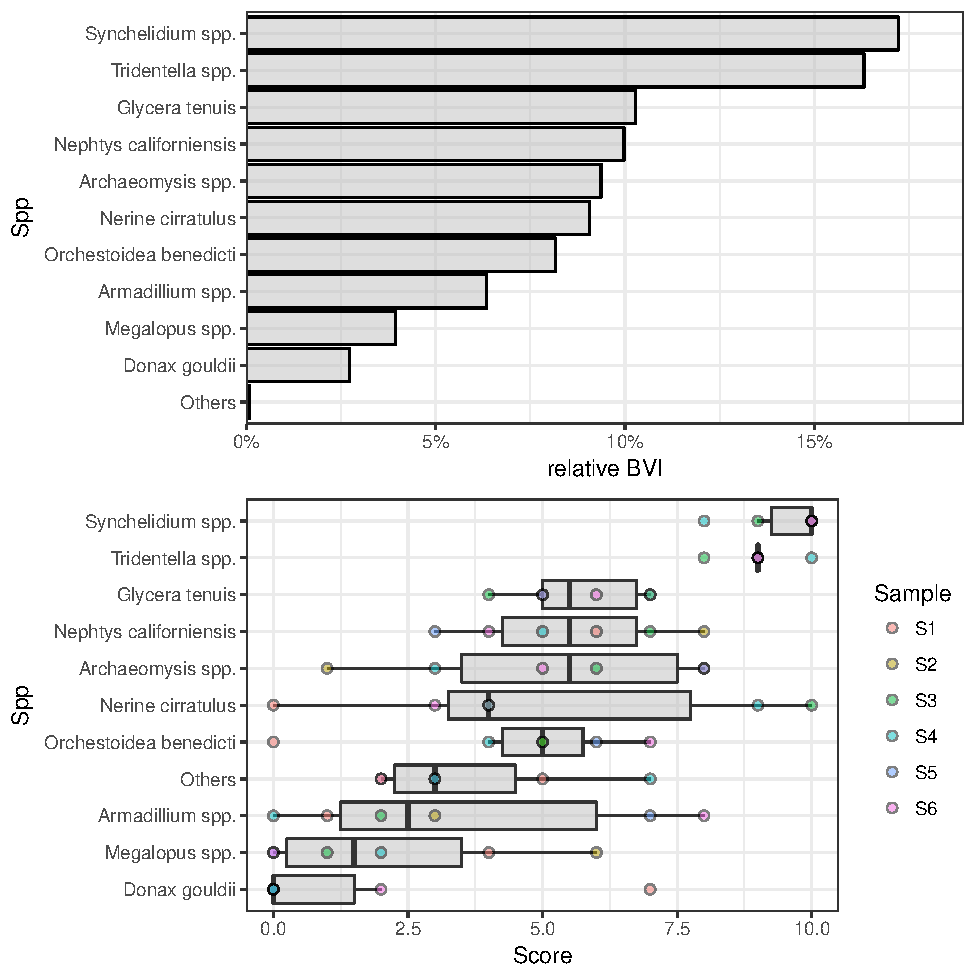
\includegraphics{BVI_Manuscript_files/figure-latex/unnamed-chunk-8-1.pdf}

\section{Discussion and Conclusions}\label{discussion-and-conclusions}

\section{References}\label{references}

\hypertarget{refs}{}

\section{Figures and Tables}\label{figures-and-tables}


\end{document}
